\documentclass{beamer}

\usetheme{Warsaw}

\usepackage[utf8]{inputenc}
\usepackage[T1]{fontenc}
\usepackage[frenchb]{babel}

\usepackage{hyperref}
\usepackage{libertine}
\usepackage{xcolor,graphicx}


\title{Sokoban LJMK}
\date{Mardi 23 avril}
\author[Lafay Gareth, Klaeyle Pierre-Louis, Mialon Laurine, Jarossay Max] {Lafay Gareth, Klaeyle Pierre-Louis, Mialon Laurine, Jarossay Max}
\institute[Université de Caen Normandie]{Université de Caen Normandie}

\setbeamertemplate{navigation symbols}{}
\setbeamertemplate{footline}[frame number]

\begin{document}

\maketitle
\frame{\tableofcontents} 

\section{Objectifs du projet}

\begin{frame} 

\begin{columns}
\begin{column}{4cm}
  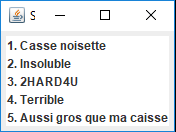
\includegraphics[scale=0.8]{MenuSoko.PNG}
\end{column}
\begin{column}{4cm}
  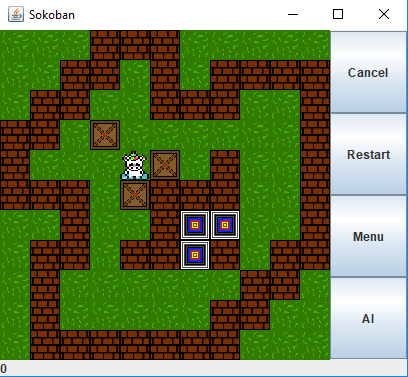
\includegraphics[scale=0.4]{JeuSoko.PNG}
\end{column}
\end{columns}

\end{frame}

\section{Architecture du projet}
\begin{frame}
\begin{column}{8cm}
  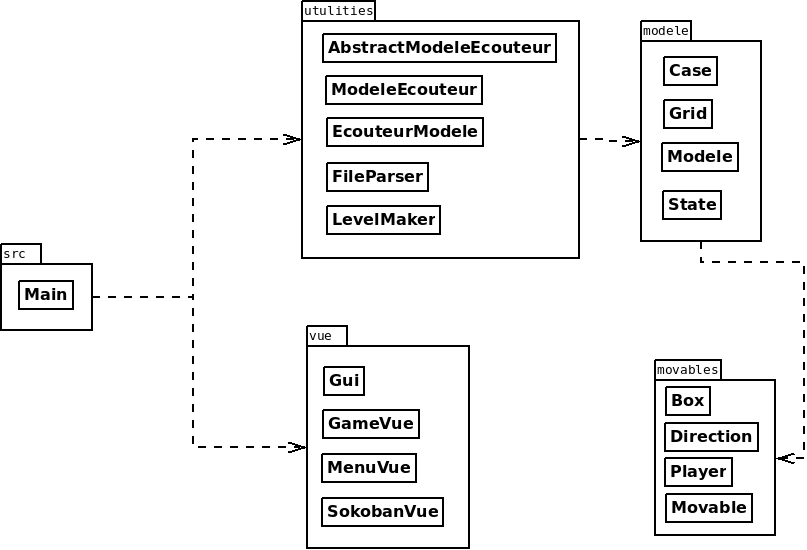
\includegraphics[scale=0.3]{Diagramme1.png}
\end{column}
\end{frame}

\section{Éléments techniques}
 

\begin{frame}
\frametitle{Description}
%\framesubtitle{Et son sous-titre}
\begin{block}{Programme}  
 \begin{itemize}
     \item Modele
     \item Vue Controleur
     \item Intelligence Artificielle
 \end{itemize}
\end{block}
\end{frame}

\begin{frame}
\frametitle{Description}
\begin{exampleblock}{Package Modele}
\hspace{2.2cm}
\begin{column}{8cm}
  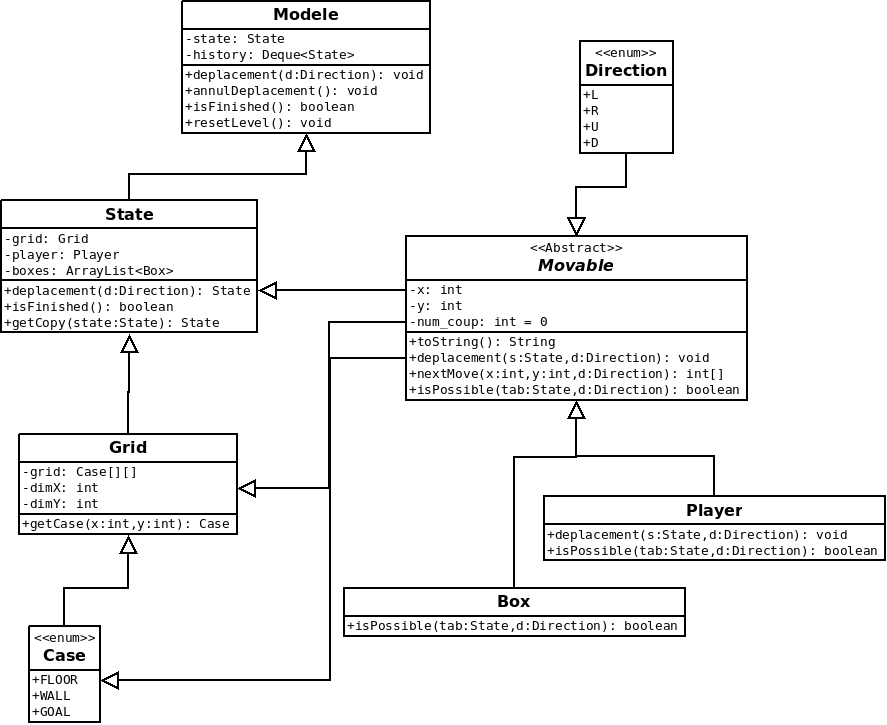
\includegraphics[scale=0.2]{Diagramme3.png}
\end{column}
\end{exampleblock}

\end{frame}

\begin{frame}
\begin{alertblock}{Bibliothèque Utilisé} 
\begin{itemize}
    \item Swing
    \item Awt
\end{itemize}
\end{alertblock}
\begin{alertblock}{Structure de donnée} 
\begin{itemize}
    \item ArrayList
    \item Enum
    \item Deque
\end{itemize}
\end{alertblock}
\end{frame}
\begin{frame}
\begin{exampleblock}{Élément Technique} 
\begin{itemize}
    \item Algorithme A*
\end{itemize}
\end{exampleblock}
\end{frame}

\section{Expérimentations et usages}
\begin{frame}
\begin{column}{8cm}
  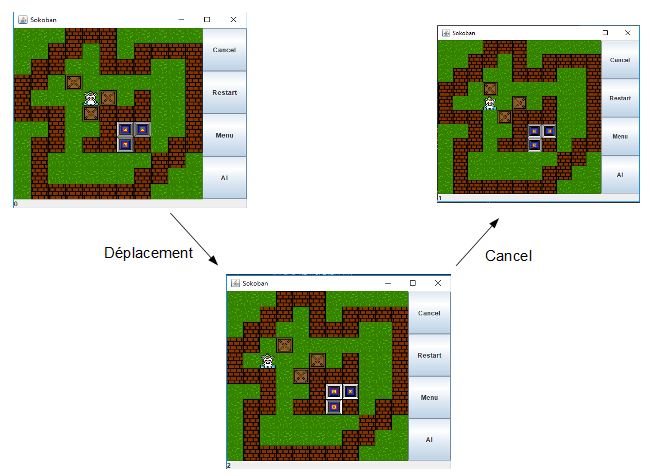
\includegraphics[scale=0.6]{Test3.PNG}
\end{column}
\end{frame}
\section{Conclusion}
  
\begin{frame}
\textbf{Conclusion}\\
 \vspace{0.8cm}
Amélioration:
\begin{itemize}
\item Nouvelle intelligence artificielle.
\item Nouveau niveau.
\item Éditeur de niveau.
\item etc ...
\end{itemize}
\end{frame}


\end{document}
